\documentclass[../main/main.tex]{subfiles}

\newdate{date}{22}{10}{2020}


\begin{document}



\marginpar{ \textbf{Lecture 7.} \\  \displaydate{date}. \\ Compiled:  \today.}


\subsection{Heterogeneous Networks}

Now, we want to understand what is the effect of \textbf{heterogeneity} in the spread of the disease. That is to say that we drop the following assumption \( k_i \sim \expval{k}  \): all \textbf{nodes are not equal} any more.

Let us consider now the \textbf{heterogeneous mean-field approximation}. Let us use a \textbf{DBMF model} and let us cut the chain at an \textbf{individual level}. This last assumption means that we consider the probability for a single individual to get the infection.
Let us follow the thread of paper \textit{“Epidemic Spreading in Scale-Free Networks”}, written by Pastor-Satorras and Vespignani. It actually provides a \textbf{SIS model on scale-free networks}. The main idea behind this paper is the following. Since nodes are not equal anymore, \textit{the probability of getting the infection strongly depends on their position (i.e. degree) in the network}. Authors' intuition is that \textbf{nodes} with \textbf{the same degree behave in the same way}. In order to do that, we need to divide the network in \textbf{degree classes}: that is to say we group together all the nodes with the same degree.


In order to write down the equations, we need to consider the number of compartments we have and introduce a density for each of them:
\begin{equation*}
  s_k = \frac{S_k}{N_k}, \qquad \rho _k = \frac{I_k}{N_k}
\end{equation*}
where \( s_k \) and \( \rho _k \) are the fractions of susceptible and infected nodes of degree \( k \) in the network. We have that \( N_k \) represents the number of nodes with degree \( k \). As before, we introduced the fractions of susceptible and infected individuals $(s_k, \rho_k)$ in the system, but in this case depending on each degree \( k \).
Obviously, the total fraction of \( \rho  \) and \( s \) in the system is: 
\begin{equation*}
    \rho = \sum_k \rho_k = \sum_k \frac{I_k}{N_k} \qquad s = \sum_k s_k = \sum_k \frac{S_k}{N_k}
\end{equation*}
While their average, sticking to the definition, is:
\begin{equation}
  \expval{\rho} = \sum_{k}^{} P(k) \rho _k, \qquad \expval{s} = \sum_{k}^{} P(k) s_k
\end{equation}

The \textbf{equation} that describes how the \textbf{probability of being infected} changes in time for the nodes that belong to the \textbf{same degree class}:
\begin{equation}
  \dv{}{t}  \rho _k (t) = - \mu \rho _k (t) + \beta k \mathcolorbox{green!20}{(1- \rho _k (t)) \Theta _k (t)}
\end{equation}
where we can distinguish as usual a "recovery" term and an "infection" term. In particular, the probability of a contact between a susceptible individual that has degree \( k \) and an infected one is highlighted in green.
This product consists in two terms: the probability for a node $i$ to be susceptible \( (1- \rho _k (t)) \) and the probability of having contact with an infected \( \Theta _k (t) \).

We want now to dwell deeper and explain better this last term. The probability that a generic node with degree \( k \) has an infected neighbor can be expressed as:
\begin{equation}
\label{eqn:theta_k(t)}
  \Theta _k(t) = \sum_{k'}^{} P(k'|k)\rho _{k'}
\end{equation}
where we sum over all the possible degree classes $k'$. In this way we expect to obtain the probability of connecting with any one of them, multiplied by the probability for that specific node to be infected.
Note, however, that we are making no assumption about the function \(  P(k'|k) \), which may change according \( k \). In principle, it could be anything, in the sense that it strongly depends on the structure of the network. However, in order to simplify the problem and derive some results, there are cases where we can make some assumptions on the structure of the latter.

Picking a node at random, the probability to be connected to a node of degree $k'$ given the node degree we start from is $k$, is the following:
\begin{equation}
  P(k'|k) = \frac{k'P(k')}{\sum_{k'} k' P(k')  } = \frac{k'P(k')}{\sum_{k} k P(k)  } = \frac{k'P(k')}{\expval{k}  }
\end{equation}
Note that \( P(k') \) is the generic probability of getting a connection at random, times \( k' \), which is the number of connections that point toward a node of degree $k'$. Finally we normalize over all possible degrees of the network \footnote{One should keep in mind that $\sum_{k} kP(k) = \sum_{k'} k'P(k')$.}. What we obtain is the probability that a generic node in the network is linked to \( k' \).  Note as \( P(k'|k) \) does not depend on \( k \).

After replacing this last result in \ref{eqn:theta_k(t)}:
\begin{equation*}
  \Theta _k (t) = \frac{\sum_{k'}k' P(k') \rho _{k'} (t)  }{\expval{k} } = \Theta (t)
\end{equation*}
Let us take a look closer to the different terms. In the numerator: there is the product between the probability that a link, randomly picked, points to a node of degree \( k' \), times the probability of being infected, Finally, we then we sum over all the possible degrees. On the other hand the expression in denominator is related only to the structure of the network. In addition, one should note that \( \Theta _k (t) \) \textbf{does not depend on} \( k \) anymore. Since we are just picking up at random it should be the same for all the nodes.

The method that we are going to exploit to \textbf{solve} the differential equation \( \dv{}{t} \rho _k (t) \) is similar to the ones previously used in other models. The first assumption is to be in the \textbf{steady state}:
\begin{equation*}
  \dv{}{t} \rho _k (t) = 0 \qquad \rightarrow  \qquad \rho _k = \frac{\beta k \Theta }{\mu + \beta k \Theta }
\end{equation*}
The next step is then to substitute the expression for \( \rho _k  \), obtained thanks to \( \Theta  \):
\begin{equation*}
    \Theta _k (t) = \frac{\sum_{k'}^{} k' P(k') \rho _{k'} (t)  }{\expval{k} } = \Theta (t) \qquad \rightarrow \qquad \Theta = \frac{1}{\expval{k} } \sum_{k}^{} \frac{k^2 P(k) \beta \Theta }{\mu + \beta k \Theta }
\end{equation*}
This is the \textbf{self consistent equation} for \( \Theta  \).



However, in order to solve this last equation, we need some workaround. First of all one should note, as what happens in statistical mechanics, this expression has different solutions depending on the value of $\Theta$:
\begin{itemize}
\item the \textbf{trivial solution} \( \Theta =0 \), that of course is not in our interest;
\item the \textbf{non trivial solution}. We can rewrite the self consistent equation as follows:
\begin{equation*}
   \Theta = \frac{1}{\expval{k} } \sum_{k}^{} \frac{k^2 P(k) \beta \Theta }{\mu + \beta k \Theta } = f(\Theta )
\end{equation*}
Hence, the solutions are the values for which it holds \( \Theta \equiv f(\Theta )\). These, geometrically, are the interceptions between the line \( \Theta  \) and the function \( f(\Theta ) \) and have to be found graphically (or using computational algorithms).

Since \( \Theta  \) is a probability, it holds that \( 0<\Theta \le 1 \). This means that, it is required for a non trivial solution to exist, the slope of \( f(\Theta ) \) must be greater than 1.
Mathematically, it means that:
\begin{equation*}
  \dv{}{\Theta }  \qty[ \frac{1}{\expval{k} } \sum_{k}^{} \frac{k^2 P(k) \beta \Theta }{\mu + \beta k \Theta } ]_{\Theta =0} \ge 1
\end{equation*}
that leads to the following condition:
\begin{equation}
\frac{\beta }{\mu \expval{k} } \sum_{k}^{}k^2 P(k) \ge 1 \qquad \rightarrow  \qquad \frac{\beta \expval{k^2} }{\mu \expval{k} } \ge 1
\end{equation}
which is the \textbf{condition} for the \textbf{existence} of an \textbf{endemic state}. Since the network has become more complex, also the structure for the condition of the endemic state acquires in complexity. Indeed, for the \textbf{epidemic threshold}:
\begin{equation}
 \frac{\beta \expval{k^2} }{\mu \expval{k} } = 1 \qquad \rightarrow \qquad \beta _c = \frac{\mu \expval{k} }{\expval{k^2} }
\end{equation}
which is pretty similar to the one previously found, but also includes a term that increases its complexity.

The first check one can make is to verify whether this last result holds also in the case of homogeneous networks. For such networks \( \expval{k^2} = \expval{k}^2   \), therefore:
\begin{equation*}
  \beta _c = \frac{\mu \expval{k} }{\expval{k^2} } = \frac{\mu }{\expval{k} }
\end{equation*}
which is exactly the expression we previously found.

\end{itemize}



Recalling what we were discussing last lectures, in \textbf{scale-free networks} with \( 2 < \gamma \le 3  \), we have \( \expval{k} \rightarrow c  \) and \( \expval{k^2}  \rightarrow \infty  \) as \( N \rightarrow \infty  \).
As the network becomes larger also its variance increases, that is:
\begin{equation*}
  \beta _c = \frac{\mu \expval{k} }{\expval{k^2} } \rightarrow 0
\end{equation*}
hence the \textbf{epidemic threshold vanishes} for \( N \rightarrow \infty  \).
This is a quite important result: \textbf{if} our \textbf{network is large enough} \textbf{every disease will spread no matter its infectivity} (see Fig. \ref{fig:07_1}). The converse is still valid: if we have disease with a very low infection rate in a small part of the network, it will not disappear if the network is large enough\footnote{Physically, we refer to this as taking the thermodynamic limit.}! That is to say we \textbf{always} find ourselves in an \textbf{endemic state}, while the threshold becomes very small. These results are actually valid for the most real epidemic models, given the networks are large enough.

\begin{figure}[h!]
\centering
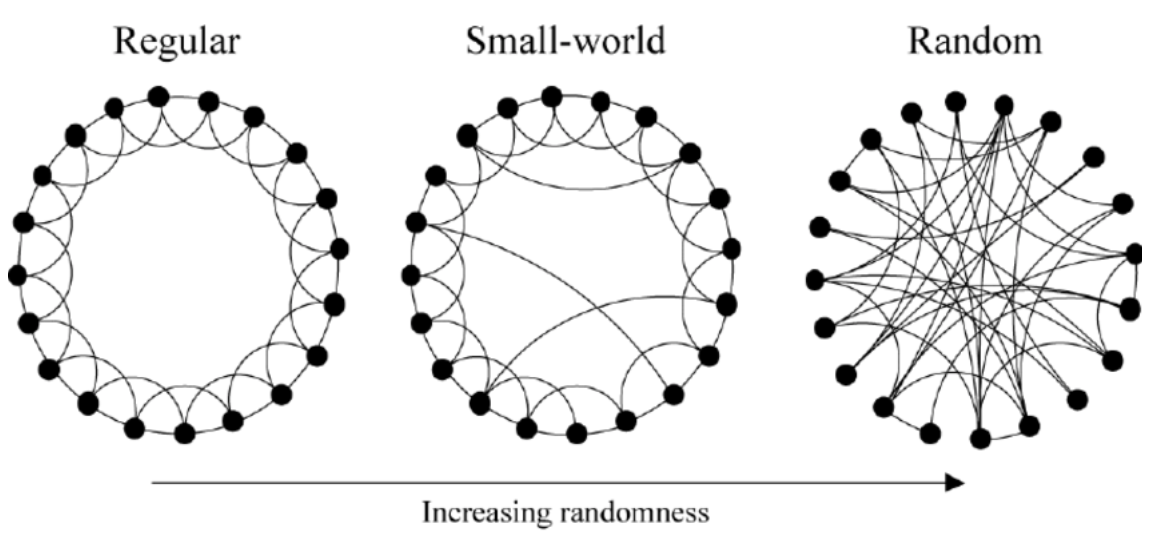
\includegraphics[width=0.6\textwidth]{../lessons/image/07/1.png}
\caption{\label{fig:07_1} In scale-free networks (and many heavy-tailed distributions) the epidemic threshold vanishes in the thermodynamic limit.}
\end{figure}

Obviously, \textbf{real networks} are not infinite: therefore we need some \textbf{finite-size corrections}. For example, we may want to derive an expression for epidemic threshold when the size of the system does not diverge.

Let us consider the degree distribution for \textbf{scale-free networks}: since the degree cannot go to infinity, it is convenient to introduce an \textbf{exponential cut-off} at some point. For instance, let us consider the air transportation network: we see that until a certain point a certain trend is followed, but then the slope of the curve starts to change and resembles to an exponential. This implies that we cannot have an infinite number of connections: the line starts out as a power law and then ends up introducing some sort of exponential cut-off. The behavior is similar to the one in Fig. \ref{fig:07_2}.

\begin{figure}[h!]
\centering
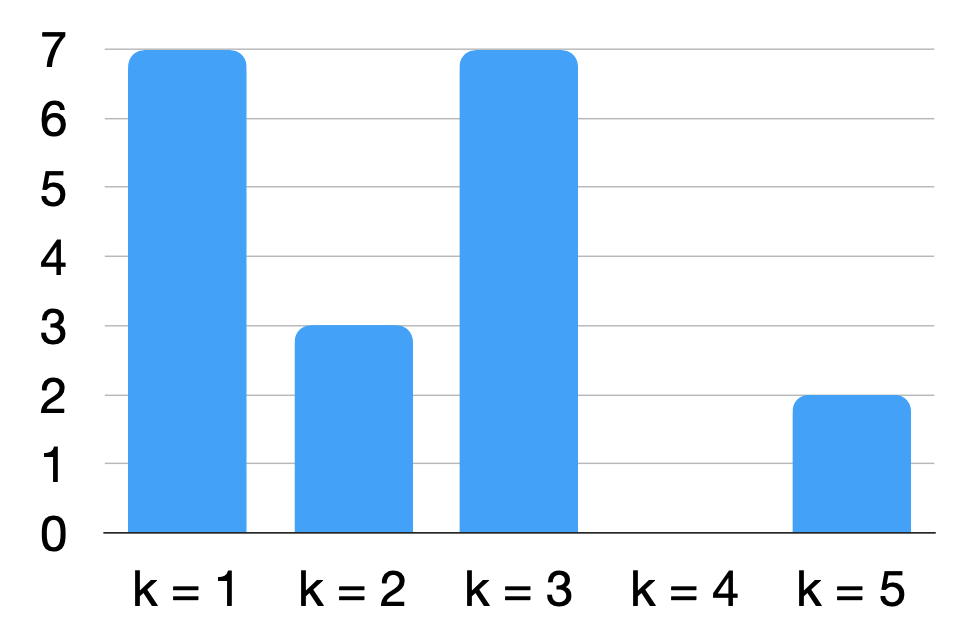
\includegraphics[width=0.7\textwidth]{../lessons/image/07/2.png}
\caption{\label{fig:07_2} Power-law with an exponential cut-off.}
\end{figure}

We introduce our considerations into our model by adding an exponential term:
 \begin{equation}
   P(K) \sim k^{- \gamma}   e^{-k/k_c}
 \end{equation}
where \( k_c \) is a \textbf{characteristic degree}.
At some point, the term we just added will become the dominant term and what happens is that, for large \( k_c \) and \( 2 < \gamma < 3  \), the epidemic threshold can be approximated as:
\begin{equation}
  \beta _c \simeq \qty(\frac{\mu k_c}{k_{min}})^{\gamma -3 }
\end{equation}
we are not going to prove the computations. However, in the lab, we will compare the epidemic thresholds for a random and for a scale-free networks in order to see how they differ. This was the last consideration about the study of the SIS model in a network.



\section{SIR model in a network}

\subsection{Degree-based mean-field theories (DBMF)}

The same as before equations can be derived for the SIR model under the assumption of \textbf{heterogeneous mean-field}. The main difference is that we need \textbf{one more equation} to take into account also the compartment related to \textbf{recovered} individuals. Their densities are \( \rho _k^S(t) \), \( \rho _k^I (t) \) and \( \rho _k^R (t) \), and it holds that \( \rho _ \infty ^R = \lim_{t \rightarrow \infty } \sum_{k}^{} P(k) \rho _k^R (t) \).
Equations take the form:
\begin{equation}
\begin{split}
  \dv{}{t} \rho _k^I (t) &= - \mu \rho _k^I (t) + \beta k \rho _k^S (t) \Gamma _k(t)  \\
  \dv{}{t} \rho _k^R (t) &= \mu \rho _k^I (t)
\end{split}
\end{equation}
with \( \rho _k^S (t) = 1 - \rho _k^I (t) - \rho _k^R (t)\) and where:
\begin{equation}
  \Gamma _k (t) = \sum_{k'}^{} \frac{k'-1}{k'} P(k'|k) \rho _{k'}
\end{equation}
is the probability of a contact with an infected node, and plays exactly the same role of \( \Theta  \) before.
Actually it represents the link from which the infection arrived to that node, however we will not show how to derive this expression beside one small consideration: the $\frac{k'-1}{k}$ term that is the main difference from the SIS model. It is present due to the fact that we cannot infect a node that has already transmitted us the disease: either because it has already recovered or because it is still infected. In this way we are taking into account that the disease is coming "from one side", therefore for us is forbidden to spread the infection towards that specific direction: recovered (or already infected) individuals cannot be infected twice.

The \textbf{epidemic threshold for random networks} results:
\begin{equation}
  \beta _c = \frac{\mu \expval{k} }{\expval{k^2} - \expval{k} }
\end{equation}
and the important thing to notice is that \( \beta _c^{SIS} \neq \beta _c^{SIR} \). This is the first time so far that the \textbf{epidemic thresholds} for these two models \textbf{differ}!

\subsection{Individual-based mean-field theories (IBMF)}

Up to now we were assuming that all the nodes with the same degree were equal. Now, since we are going to study the \textbf{individual based mean-field} theories, we will not consider a specific instance of the network, but an average over all the possible networks we can obtain \textbf{given} that \textbf{degree distribution}.
That is to say, that under the \textbf{Heterogenous Mean-Field framework} we are solving the epidemics problem for an \textbf{ensemble of networks} whose common feature is the degree distribution \( P(k) \)\footnote{the so called "ensemble" of networks!}.

In the degree based approach we previously assumed that all the nodes with the same degree to be equal. We were therefore analyzing not a specific instance of networks, but its \textit{average}. This is actually what in physics we refer as \textbf{annealed networks}.
On the opposite, we call \textbf{quenched networks} when we consider a \textit{particular realization} of one network. The idea is really simple: instead of considering the average, we consider a particular instance network. This is the main difference between a degree based (i.e. annealed networks) or an individual based approach (i.e. quenched networks).

Let us write down the equations for the \textbf{quenched mean-field}. We are going to introduce a \textbf{discrete time} framework in order to make equation simpler. However, nothing prevents us to use differential equations, where time is a continuous variable.

Let us consider \( \rho _i (t) \), that is the probability for node $i$ of being infected at time \( t \). The total fraction of infected individuals is given by \( \rho (t) = \sum_{i}^{} \rho _i (t)   \).\\
At the following time-step, the probability of being infected at time \( t+1 \) is:
\begin{equation}
  \rho _i (t+1) = \mathcolorbox{green!20}{\rho _i(t) (1- \mu )} + \mathcolorbox{yellow!40}{(1 - \rho _i(t))q_i(t)}
  \label{eqn:SIR_IBMF}
\end{equation}
which is the sum of the probability of being infected and not get cured (green term) and the probability of being susceptible multiplied by the probability of contracting the disease (yellow term).\\
We now need an expression for \( q_i(t) \), that is the \textbf{probability} for node \( i \) to \textbf{be infected by, at least, one neighbour}. The basic idea for doing this is:
\begin{equation}
  q_i (t) = 1 - \prod_{j=1}^{N} \qty[1- \beta A_{ij} \rho _j (t)]
\end{equation}
Let us consider Fig. \ref{fig:07_3}, in green we have susceptible nodes, which include node \( i \) itself, and in red its infected neighbours.
The probability of getting infected, at least, by a generic node $j$ is:
\begin{equation}
   \beta A_{ij} \rho _j (t) 
\end{equation}
Its complementary to 1 is the probability of $NOT$ get the infection by node $j$.  
\begin{equation}
   [1- \beta A_{ij} \rho _j (t)] 
\end{equation}
Repeating this argument for all neighbors that are actually infected, we can obtain the probability of $NOT$ contracting the disease from $ANY$ neighbor, namely:
\begin{equation}
    \prod_{j=1}^{N} [1- \beta A_{ij} \rho _j (t)]
\end{equation}
Again, we previously introduced \(   q_i (t) \) as the \textbf{probability of getting infected by at least one neighbor}. Finally, the probability of getting infected is the \textit{complementary} to one of the probability of not getting infected by \textit{any} neighbor:
\begin{equation}
  q_i (t) = 1 - \prod_{j=1}^{N} \qty[1- \beta A_{ij} \rho _j (t)]
\end{equation}

\marginpar{
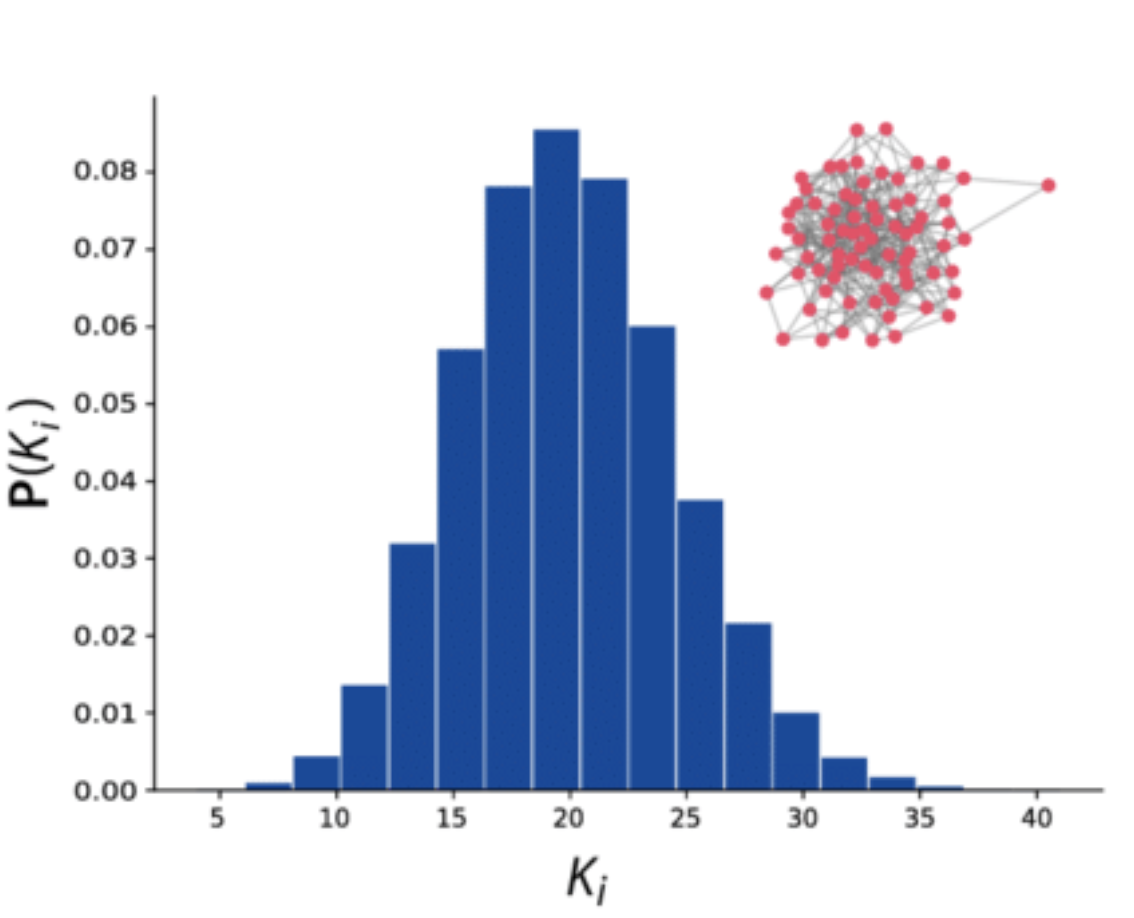
\includegraphics[width=\marginparwidth]{../lessons/image/07/3.png}
\captionof{figure}{\label{fig:07_3} In green susceptible nodes, while in red the infected neighbours.}
}

Note as the system of (\( \rho _i (t+1) \)) equations can be solved numerically by iteration. This results to be precise for the entire epidemic diagram, and faster than numerical simulations: there is no need of averages and reproduces individual nodes probabilities. Indeed, in this framework we will obtain two equations for each of the nodes: we have \( 2^N \) equations, where \( N \) is the size of the system.

\begin{remark}
One should have noted that this last approach differs from the degree based mean field theories by the fact that now we are including adjacency matrix \( A_{ij} \), while before we took only the average.
\end{remark}
The equation (\ref{eqn:SIR_IBMF}) therefore takes the form:
\begin{equation}
      \rho _i (t+1) = \rho _i(t) (1- \mu ) + (1 - \rho _i(t))\left(1 - \prod_{j=1}^{N} \qty[1- \beta A_{ij} \rho _j (t)]\right)
  \label{eqn:SIR_IBMF}
\end{equation}

We can also \textbf{solve analytically} the system at the \textbf{steady state} in order to estimate the \textbf{epidemic threshold}. Assuming that we find ourselves in the steady state:
\begin{equation*}
  \lim_{t \rightarrow \infty } \rho _i (t) = \rho _i ^* \quad \rightarrow \quad \rho _i (t+1) = \rho _i (t) = \rho _i^*
\end{equation*}
it follows that:
\begin{equation}
\label{eqn:mu_rho_i^steady}
  \mu \rho _i^* = (1- \rho _i^*) q_i^* \quad \rightarrow \quad q_i^* = 1 - \prod_{j=1}^{N} \qty[1- \beta A_{ij} \rho _j^*]
\end{equation}

Now, if we think about what happens when we are in \textbf{proximity of the epidemic threshold} (\textit{epidemic onset}), it happens that \( \rho _i^* \) can be assumed to be small for all the nodes \( \rho _i^* = \varepsilon _i^* \ll 1 \).
Therefore, the product in \( q_i^* \) can be approximated by a sum:
\begin{equation}
\label{eqn:q_prod}
  q_i^* = 1 - \prod_{j=1}^{N} \qty[1- \beta A_{ij} \varepsilon _j^*] \simeq \beta \sum_{j=1}^{N} A_{ij} \varepsilon _j^*
\end{equation}
Substituting what we have just found in the lhs of \ref{eqn:mu_rho_i^steady} we obtain:
\begin{equation}
  \mu \varepsilon _i^* = \beta (1- \varepsilon _i^*) \sum_{j=1}^{N} A_{ij} \varepsilon _{j}^*
\end{equation}
that is a linear system where the interaction is given by the adjacency matrix:
\begin{equation*}
  \mu \varepsilon _i^* = \beta \sum_{j=1}^{N} A_{ij} \varepsilon _{j}^* - \cancel{ \beta \varepsilon _i^* \sum_{j=1}^{N} A_{ij} \varepsilon _{j}^* }
\end{equation*}
Neglecting second order terms, we have that:
\begin{equation}
  \frac{\mu }{\beta } \varepsilon _i^* = \sum_{j=1}^{N} A_{ij} \varepsilon _j^*
\end{equation}
This linear system has solution only if \( \frac{\mu }{\beta } \) is an \textbf{eigenvalue} of the \textbf{adjacency matrix} \( A_{ij} \). Here we should understand why last lecture we stated that the spectrum of the adjacency matrix is something we may be interested in.
Hence:
\begin{equation}
  \beta = \frac{\mu }{\Lambda _i}
\end{equation}
where \( \Lambda _i \) is a generic eigenvalue of the adjacency matrix \( A_{ij} \). However, since we are interested in the \textbf{smallest} possible \textbf{value} of \( \beta  \) for which there exists solution, we need to take the \textbf{largest eigenvalue} of the adjacency matrix \( A \):
\begin{equation}
  \beta _c = \frac{\mu }{\Lambda _{max}}
\end{equation}
The last one is the \textbf{expression} for the \textbf{epidemic threshold}, and it is a \textbf{general result} that is valid not only while using this approximation, but for a more general framework in a generic network.


\subsection{DBMF vs IBMF: Epidemic treshold}
One may wonder now what is the relation between the two values for the epidemic thresholds we have found for the different mean-field theories, that is DBMF and IBMF. We have found that:
\begin{itemize}
\item for \textbf{DBMF}:
\begin{equation*}
  \beta _c^{DBMF} = \frac{\mu \expval{k} }{\expval{k^2} }
\end{equation*}

\item for \textbf{IBMF}:
\begin{equation*}
\beta _c^{IBMF} = \frac{\mu }{\Lambda _{max}}
\end{equation*}
\end{itemize}
For \textbf{scale-free networks} \( P(k) \sim k^{-\gamma  } \) it holds that:
\begin{equation}
  \Lambda _{max} \sim \max \qty(\sqrt{k_{\max}}, \frac{\expval{k^2}}{\expval{k}}   )
\end{equation}
And in particular:
\begin{equation}
\beta _c \sim
  \begin{cases}
   \mu / \sqrt{k_{\max}} & \gamma > 5/2  \\
   \mu \expval{k}/\expval{k^2} & 2 < \gamma < 5/2
  \end{cases}
\end{equation}
We can conclude that \textbf{IBMF} is \textbf{more accurate} than DBMF. Due to the approximation, indeed, the \textbf{DBMF} is  \textbf{accurate only} in the \textbf{proximity of the epidemic threshold}, while IBMF is accurate for the entire epidemic diagram.

\end{document}
